\documentclass{article}
\usepackage{ctex}
\usepackage{amsmath}
\usepackage{listings}
\usepackage[top=2cm]{geometry}
\lstset{language=C++,tabsize=3}
\usepackage{graphicx}
\graphicspath{{picture/}}

\title{寻找二叉树最短路径}
\author{W.J.Z}
\date{}

\usepackage{fancyhdr}
\pagestyle{fancy}
\lhead{}
\chead{}
% bfseries
\lhead{\bfseries W.J.Z copyright reserved }
\rhead{\bfseries https://blog.csdn.net/Leader\_wang}

\begin{document}
	\maketitle
	为了增强自己的工程能力,我每天在牛客网上code一个算法题,虽然一天一个,但坚持下来就会积累很多,现在把我的结题思路记录下来分享。
	\section{问题}
	
	Given a binary tree, find its minimum depth.The minimum depth is the number of nodes along the shortest path from the root node down to the nearest leaf node.
	
	中文:给一个二叉树,找出最短路径的深度。
	\section{结题思路}
	大部分人看到这立马想到二叉树的遍历算法,采用递归函数求出二叉树的最短路径。这种算法即耗内存又耗时间,而采用层次遍历就是一种不错的方法,但如何实现最短路径叶子的辨别和层次深度增加的计算?
	\begin{enumerate}
		\item 最短路径叶子识别:其实很简单,遇到的第一个无左右儿子的节点即为最短路径叶子节点。
		\item 层次深度计算:depth表示当前层次遍历的深度,length表示当前层次还没有遍历节点的总个数:等length==0时说明当前层次已经遍历完毕,depth可以加1,同时将下一层节点总数count值赋予length进行下一层遍历,count值重新为0。count用来计算当前遍历层次下一层的节点数,只要当前遍历的节点至少有一个子节点就可加1,否则返回depth。
		考虑最开始的情况:第0层的剩余遍历节点数为0,即length=0;第一层的节点总数为1,即count=1;
	\end{enumerate}
	\begin{figure}
		\centering
		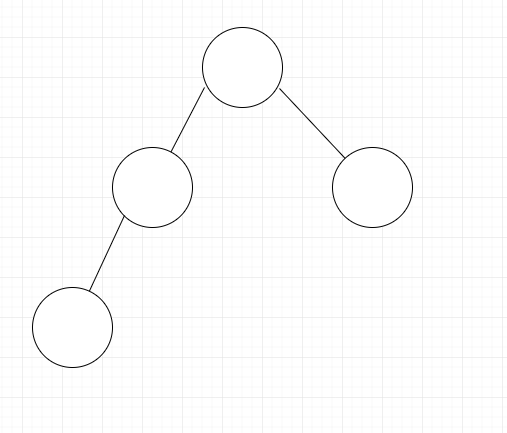
\includegraphics[width=0.2\textwidth]{1}
		\caption{二叉树}
	\end{figure}
	
	\section{C++代码}
	二叉树层次遍历使用队列容器,很好理解。
	\begin{lstlisting}
	class Solution {
		public:
		int run(TreeNode *root) {
			int depth = 0,length=0,count=1;
			TreeNode *temp,*p ;
			queue<TreeNode*> que;
			if(root==NULL)
				return depth;
			p=root;
			que.push(p);
			while(!que.empty())
			{
				if(length==0)
				{
					depth++;length=count;count=0;
				}
				else
				{
					temp = que.front();
					que.pop();
					length--;
					if(temp->left!=NULL)
					{
						que.push(temp->left);
						count++;
					}
					if(temp->right!=NULL)
					{
						que.push(temp->right);
						count++;
					}    
					if(temp->left==NULL&&temp->right==NULL)
						return depth;
				}
			}
		return depth;}};
	\end{lstlisting}
	\section{运行效果}
	\begin{figure}[h]
		\centering
			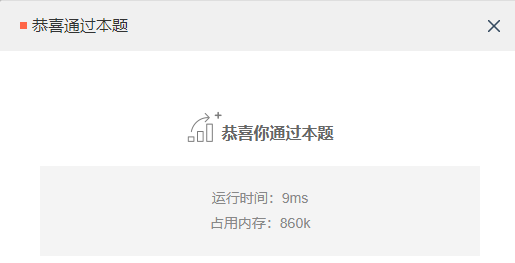
\includegraphics[scale=0.6]{2}
			\caption{层次遍历}
	\end{figure}
		\begin{figure}[h]
		\centering
		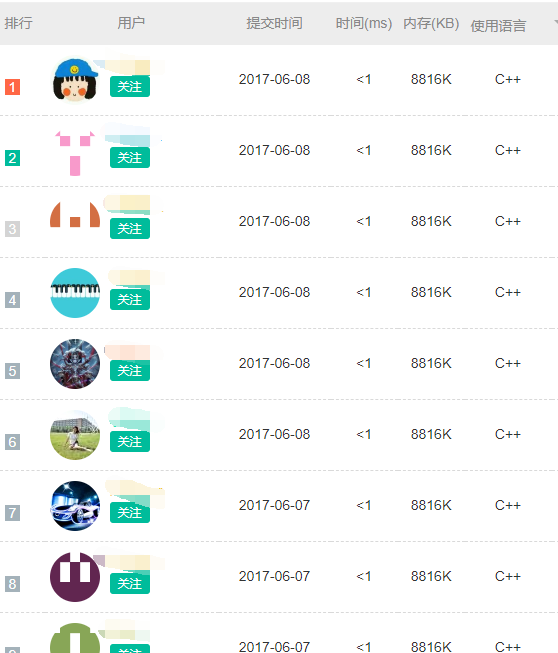
\includegraphics[scale=0.4]{3}
		\caption{递归遍历}
	\end{figure}
\end{document}